\section{Where can Bioinformatics Help?}

\subsection{Databases and Tools for Analysis}

\begin{frame}[c]{Available Databases are Decentralized}
    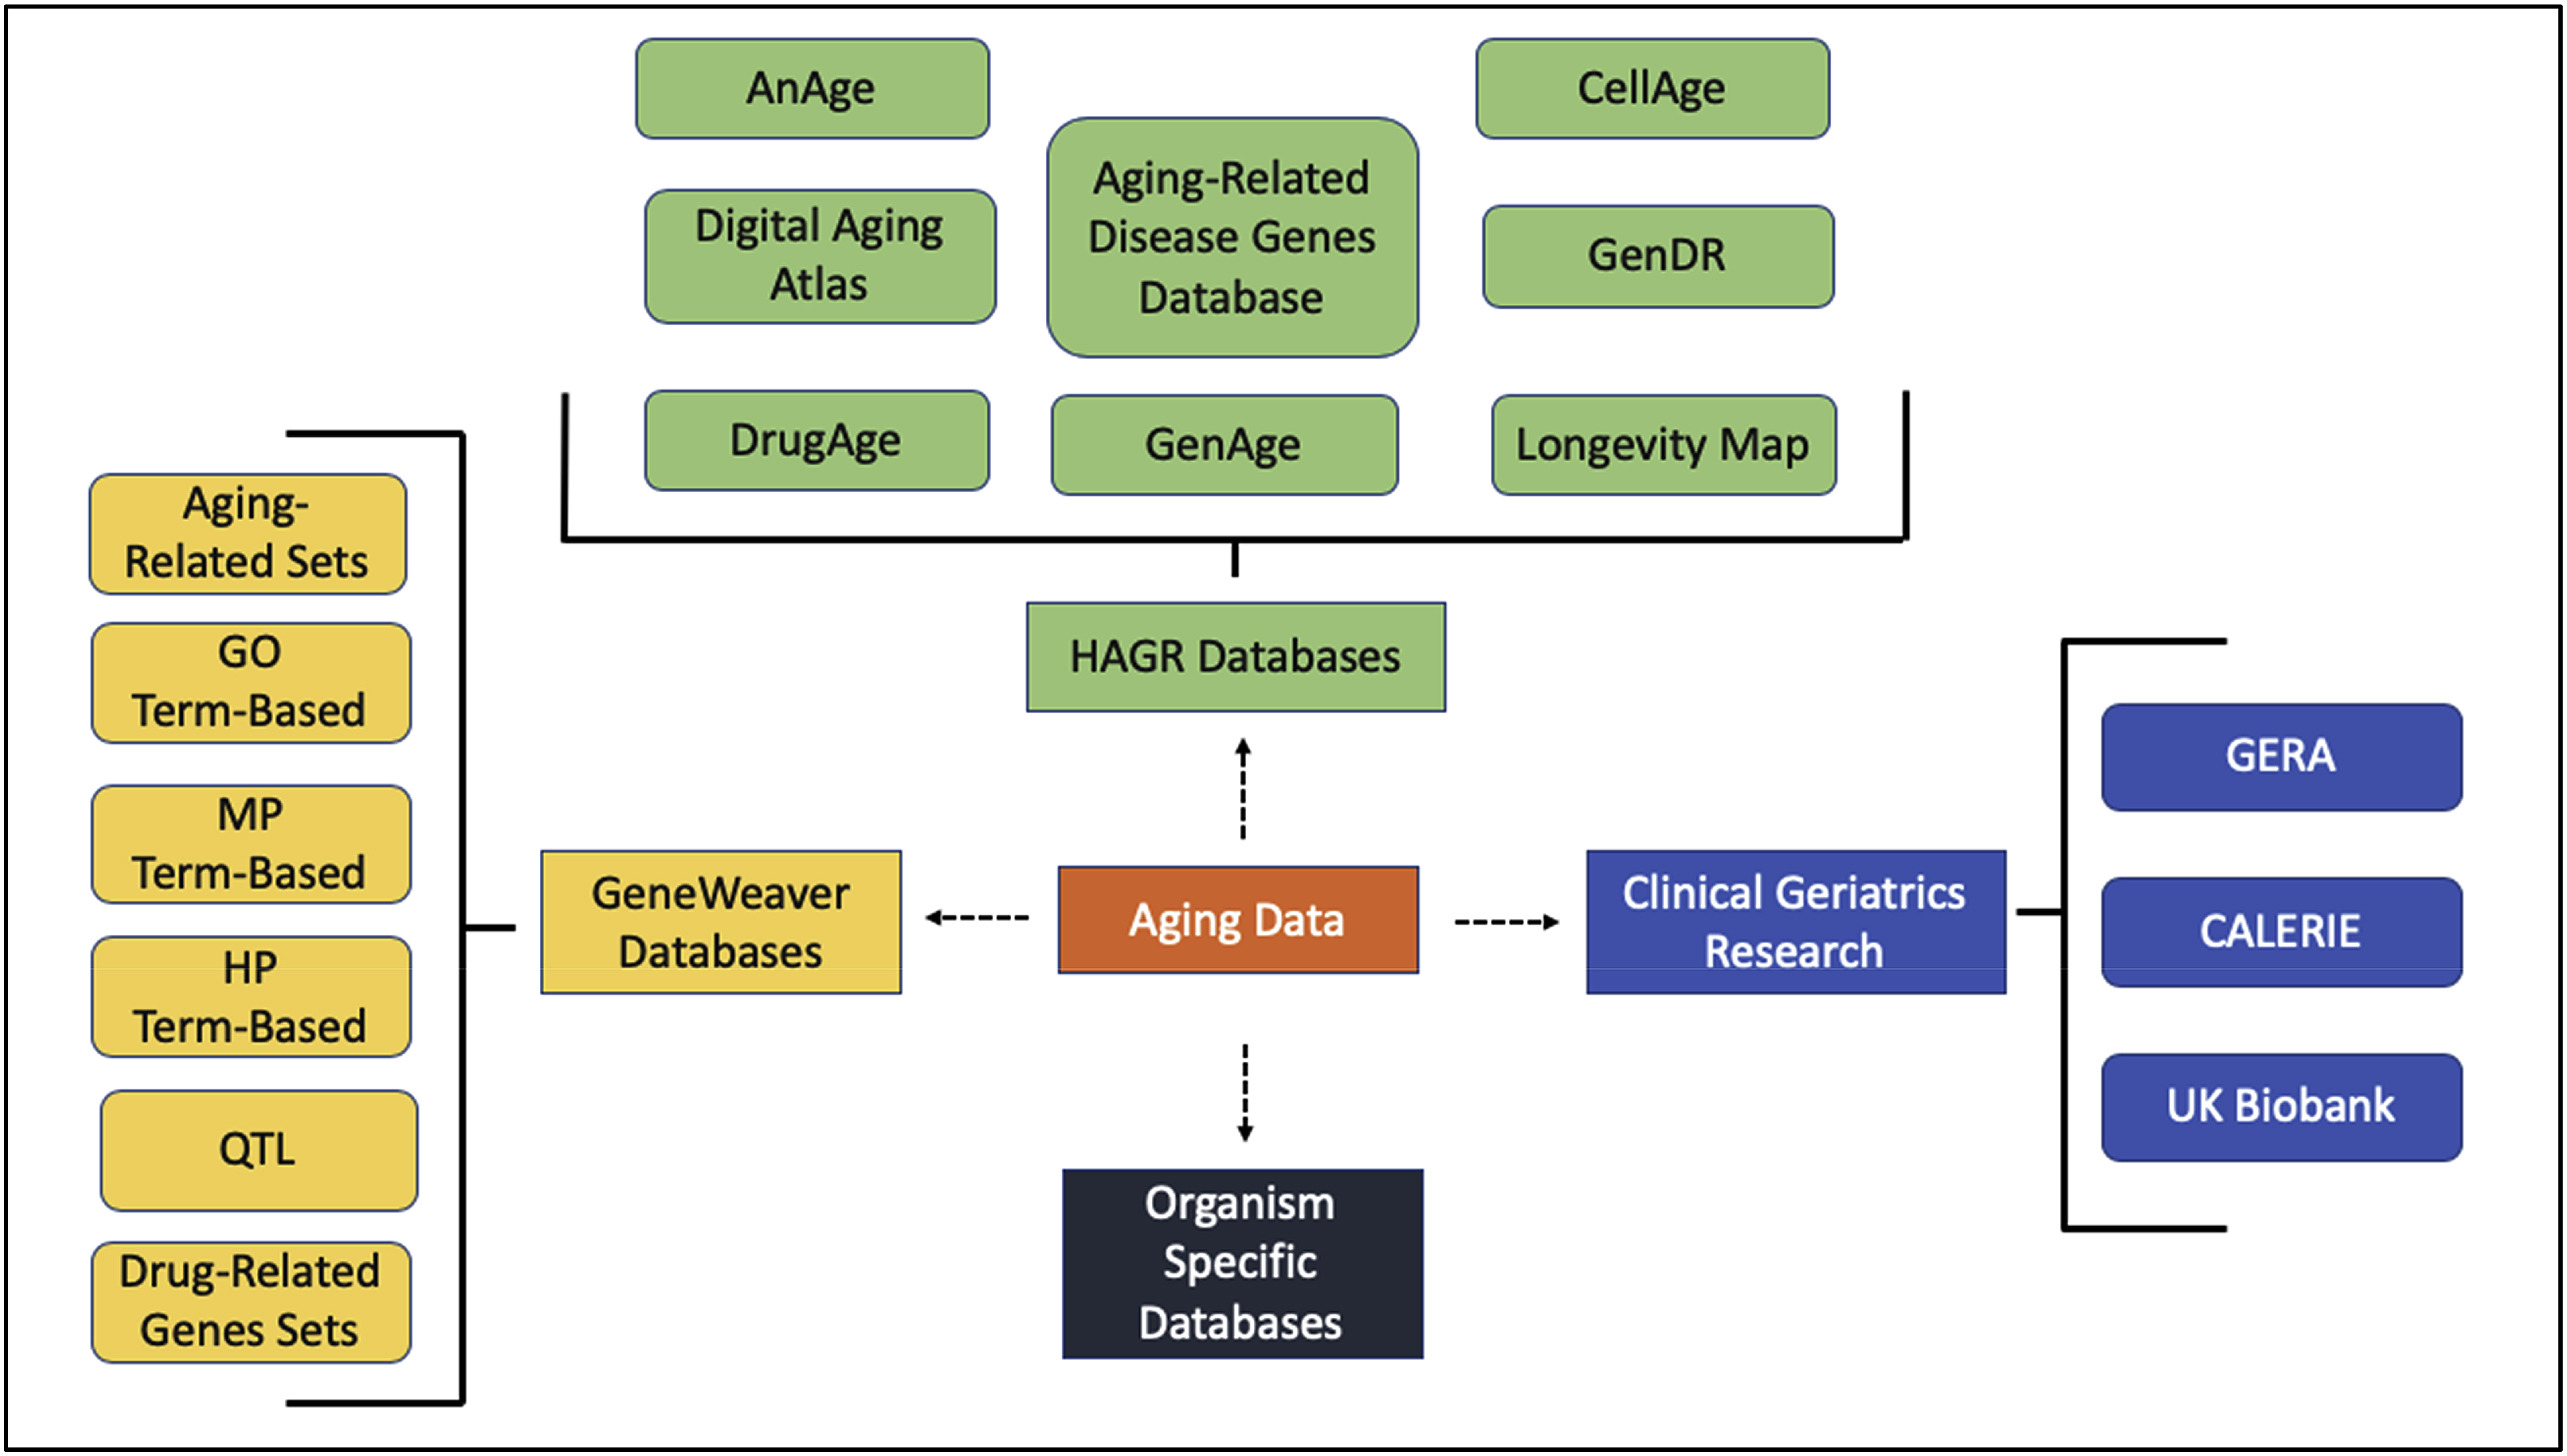
\includegraphics[width=\textwidth]{bioinfo_databases} \\
    Source: \cite{kruempel2019computational}
\end{frame}


\begin{frame}[c]{Computational Tools}
    \begin{itemize}[<+(1)->]
        \item Prism - statistical analysis and graphing program
        \item Online Application for Survival Analysis (OASIS) - online tool for statistical analysis of lifespan data
        \item R packages: `survival`, `flexsurf`, `survminer` - rapid generation of survival curves and statistical analysis
        \item Machine Learning approaches - gene classification, mortality related biomarker and gene expression profile identification
    \end{itemize}
    Source: \cite{kruempel2019computational}
\end{frame}


\begin{frame}[c]{Areas for Improvement}
    \large
    \begin{itemize}[<+(1)->]
        \item Centralized access to Databases - making study data available for further analysis in a {\em centralized} manner
        \item Increased Biobank usage - collecting biological and clinical data on representative populations
        \item Sophisticated Tools for Analysis - for the next tier of qualitative analysis 
        \item Standardization - for easier access and interoperability
    \end{itemize}
\end{frame}

\subsection{Machine Learning}

\begin{frame}[c]{Machine Learning}
    \large
    \begin{itemize}[<+(1)->]
        \item Classifying genes and proteins into aging or non-aging-related
        \item Classifying genes in model organisms as pro- or anti-longevity
        \item Prediction of aging-related genes
        \item Identification of improved biomarkers for aging in humans
        \item Establishing aging- and mortality-related gene expression profiles in humans
    \end{itemize}
    \footnotesize
    According to \cite{kruempel2019computational}, \cite{putin2016deep}, \cite{townes2020identifying}, \cite{kerber2009gene}, \cite{nakamura2007method}
\end{frame}


% \begin{frame}[c]{Analysis}
%     \large
%     Large datasets, ever-more data
%
%     \begin{itemize}[<+(1)->]
%         \item Every medical database getting larger (picture would be great)
%         \item Countries started biobanks (Denmark, UK, ...) (check for source)
%         \item No one attempts analysis: no one has appropriate tools!
%         \item needed: correlating genes with injuries/health problems/allergies over lifetime
%         \item new tools, new bigger better software and comp capacity
%     \end{itemize}
% \end{frame}


% \subsection{Simulation}

% \begin{frame}[c]{Simulation}
%     current Pharmaceutical battle: better simulator (find source with details or picture)
% \end{frame}

% \begin{frame}[c]{Simulation II}
%     AlphaFold2 and others are getting better and better
% \end{frame}

% \begin{frame}[c]{Simulation: Impact}
%
%     \begin{itemize}[<+(1)->]
%         \item cheaper preliminary analysis
%         \item identification of missing or additional effect pathways
%         \item faster research iterations
%     \end{itemize}
% \end{frame}
